\chapter{Bag of Visual Words}
\section{Image classification pipeline}
In order to implement image classification, we need two major components:
\begin{itemize}
    \item A way to describe images. Not just local features descriptors, but a \textbf{global} representation of the image.
    \item A procedure to \textbf{compare} different images and learn a statistical model of a specific class. 
\end{itemize}

\subsection{Nearest Neighbor classifier}
The simplest way to \textit{learn} a model of a specific class is by using nearest neighbor technique.\newline\newline
Let's assume that we have just two classes (binary classification problem) and that we represented our training images into a feature space. The idea is to classify a new test image with the label of the closest training image (e.g. in terms of Euclidean distance) in the feature space.\newline\newline
This method has some problems:
\begin{itemize}
    \item If the test image is equally distant from two (or more) neighbors, a discriminant is needed for classification.
    \item It is very sensitive to outliers.
\end{itemize}
\subsection{k-Nearest Neighbors classifier}
A better generalization of the previous technique is the k-Nearest Neighbors classifier.\newline\newline
The image is assigned to the most common class among its k nearest neighbors (k is a positive integer, typically small). if k = 1, the method is equal to the Nearest Neighbor classifier.\newline\newline
This method solves the problems described before but it still has weakness. If k is too large and the dataset is too small, the model will be highly biased by the most frequent class. So, in order to work well, k-NN needs large datasets.
\section{Simple image representation}
The simplest representation is provided by raw pixels. We need to map all the images, despite the resolution, to the same dimensional feature space. Then we can represent images as a 2D or 1D array of pixels, define a distance (e.g. L1 or L2) to compare images and use k-NN for classification.\newline\newline
The L1 distance metric is defined as follows:
\[d_{L1}(I_{1}, I_{2}) = \sum_{p}|I_{1}^{p} - I_{2}^{p}|\]
\[ \begin{bmatrix}
    56 & 32 & 10 & 18\\
    90 & 23 & 128 & 133\\
    24 & 26 & 178 & 200\\
    2 &  0  & 255 & 220\\
\end{bmatrix}
-
\begin{bmatrix}
    10 & 20 & 24 & 17\\
    8  & 10 & 89 & 100\\
    12 & 16 & 178& 170\\
    4  & 32 & 233& 112\\
\end{bmatrix}
=
\begin{bmatrix}
    46 & 12 & 14 & 1\\
    82 & 13 & 39 & 33\\
    12 & 10 & 0 & 30\\
    2 & 32 & 22 & 108\\
\end{bmatrix}
\rightarrow
456
\]
Following this pipeline, we obtain a model that is fast for training (it just only needs to memorize training data for k-NN) but slow for predictions, because it needs to compute the distance, for each test image, between the current image and all the training images. This is bad because the goal is to find a model that has slow training time and fast prediction time.\newline\newline
A better result can be achieved by doing the following things:
\begin{itemize}
    \item Use a better image representation
    \item Rely on better functions to compare images
    \item Use better classifiers
\end{itemize}
\section{Bag of Visual Words}
Bag Of Visual Words is a technique to describe images. The approach has its origin in text retrieval and it is an extension of the Bag of Words algorithm. In Bag Of Words, we scan through the entire document and keep a count of each word appearing in the document. Then, we create a histogram of frequencies of words and use it to describe the text document. In Bag Of Visual Words, our input are images and we use \textbf{visual words} to describe them.
\newline\newline
The pipeline follows these steps:
\begin{enumerate}
    \item Extract local features (e.g. using SIFT) from training images.
    \item Quantize the feature space (build a visual dictionary or codebook). Make this operation via clustering algorithms such as K-means. The center points, that we get from the clustering algorithm, are our visual words.
    \item For each feature of each training image, find the closest visual word in the visual dictionary and build frequency histograms (one for each training image).
    \item Compute histograms of visual words of \textbf{test} images (following the same procedure) and predict their class using the histograms of training images (e.g. using k-NN).
\end{enumerate}
\subsection{Feature extraction}
Note that features extracted using SIFT will be mostly around the object, so, in some cases it could be a better idea to use a feature extraction algorithm that takes into account also the background (e.g. even random sampling).
\subsection{Visual dictionary}
After the feature extraction step, we have a list of feature descriptors (e.g. SIFT descriptors) that contains the descriptors of all the images. These descriptors are used as input of a clustering algorithm such as k-means. This algorithm forms k clusters and returns the center of each group. Each cluster center is a visual word and all these k visual words form the visual dictionary.\newline\newline
\textbf{k-means clustering:} The goal is to minimize sum of square Euclidean distances between points $x_{i}$ and their nearest cluster centers $m_{k}$
\[D(x,m) = \sum_{k}\sum_{i \in k}(x_{i} - m_{k})^{2}\]
Application of Lloyd's algorithm:
\begin{enumerate}
    \item Randomly initialize $\textbf{K}$ cluster centers
    \item Iterate until convergence
    \begin{enumerate}
        \item Assign each data point to the nearest center
        \item Recompute each cluster center as the mean of all points assigned to it
    \end{enumerate}
\end{enumerate}
How to choose the parameter $K$ of the algorithm?
\begin{itemize}
    \item Too small: visual words not representative of all patches.
    \item Too large: quantization artifacts, overfitting.
\end{itemize}
\subsection{Create histograms}
At this point, we create histogram of visual words of each image. This assignment step can be done in two ways:
\begin{itemize}
    \item \textbf{Hard assignment:} For each feature in the image, find the closest visual word in the visual dictionary and increase by one the count of that particular word.
    \item \textbf{Soft assignment:} Weigh frequent and infrequent words differently. A visual word that appears often is less useful for matching, so it will have a small weight attached to it. On the other hand, an infrequent word will have a bigger weight.\newline\newline
    This concept is inherited from Bag of Words for text retrieval. Instead of computing regular histogram distance, we weight each word by its inverse Document Frequency such as:
    \begin{center}
        IDF of word $j$: log ( \textit{number of documents / number of documents in which $j$ appears)}
    \end{center}    
\end{itemize}
\subsection{Classification}
After creating histograms of visual words both for testing and training images, use any classification model (k-NN, SVM, ...) to perform classification. 

\subsection{Spatial information}
In Bag of Visual Words spatial information is lost. In order to reintroduce it, we can use spatial pyramids. Instead of having one-level histogram, we iterate the procedure at different levels of spatial resolution.
\begin{itemize}
    \item Pyramid is built by using multiple copies of the image.
    \item Each level is 1/4 of the size of the previous level.
    \item The lowest level is the one with the highest resolution.
    \item The highest level is the one with the lowest resolution.
\end{itemize}
\begin{center}
    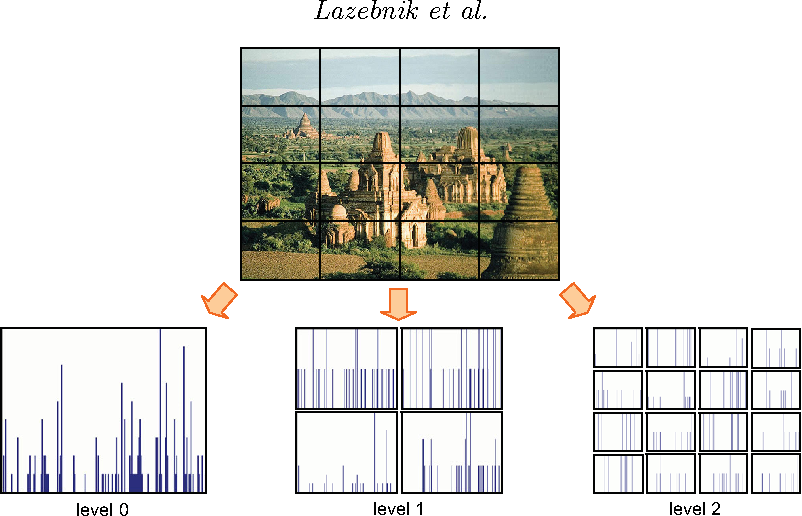
\includegraphics[scale = 0.4]{images/Spatial pyramids.png}
\end{center}

